
%(BEGIN_QUESTION)
% Copyright 2013, Tony R. Kuphaldt, released under the Creative Commons Attribution License (v 1.0)
% This means you may do almost anything with this work of mine, so long as you give me proper credit

Suppose an instrument technician needs to connect a loop-powered 4-20 mA pressure transmitter to the input of a loop controller, and does so like this:

$$\includegraphics[width=15.5cm]{i02282x01.eps}$$

Explain what is wrong with this circuit, and what is needed to fix the problem.

\underbar{file i02282}
%(END_QUESTION)





%(BEGIN_ANSWER)

Right now the circuit consists of two electrical {\it loads} and no {\it source(s)}.  Since both the controller (with a 250 ohm resistor) and the transmitter require an external power supply, we must connect a DC voltage source in series with both to provide the power necessary to generate a 4-20 mA current signal:

$$\includegraphics[width=15.5cm]{i02282x02.eps}$$

%(END_ANSWER)





%(BEGIN_NOTES)


%INDEX% Pictorial circuit review (4-20 mA loop)

%(END_NOTES)


